\documentclass{article}%
\usepackage[T1]{fontenc}%
\usepackage[utf8]{inputenc}%
\usepackage{lmodern}%
\usepackage{textcomp}%
\usepackage{lastpage}%
\usepackage[head=40pt,margin=0.5in,bottom=0.6in]{geometry}%
\usepackage{graphicx}%
%
\title{\textbf{Comunidades de Trujillo protestan por falta de gas desde hace cuatro meses}}%
\author{El Nacional Web}%
\date{06/12/2018}%
%
\begin{document}%
\normalsize%
\maketitle%
\textbf{URL: }%
http://www.el{-}nacional.com/noticias/protestas/comunidades{-}trujillo{-}protestan{-}por{-}falta{-}gas{-}desde{-}hace{-}cuatro{-}meses\_262344\newline%
%
\textbf{Periodico: }%
EN, %
ID: %
262344, %
Seccion: %
Protestas\newline%
%
\textbf{Palabras Claves: }%
Servicios, Agua, Protestas, Trujillo\newline%
%
\textbf{Derecho: }%
2.8%
, Otros Derechos: %
NO\_TIENE%
, Sub Derechos: %
2.8.1%
\newline%
%
\textbf{EP: }%
SI\newline%
\newline%
%
\textbf{\textit{Los manifestantes también reclaman por el agua, el alumbrado y el estado de las calles}}%
\newline%
\newline%
%
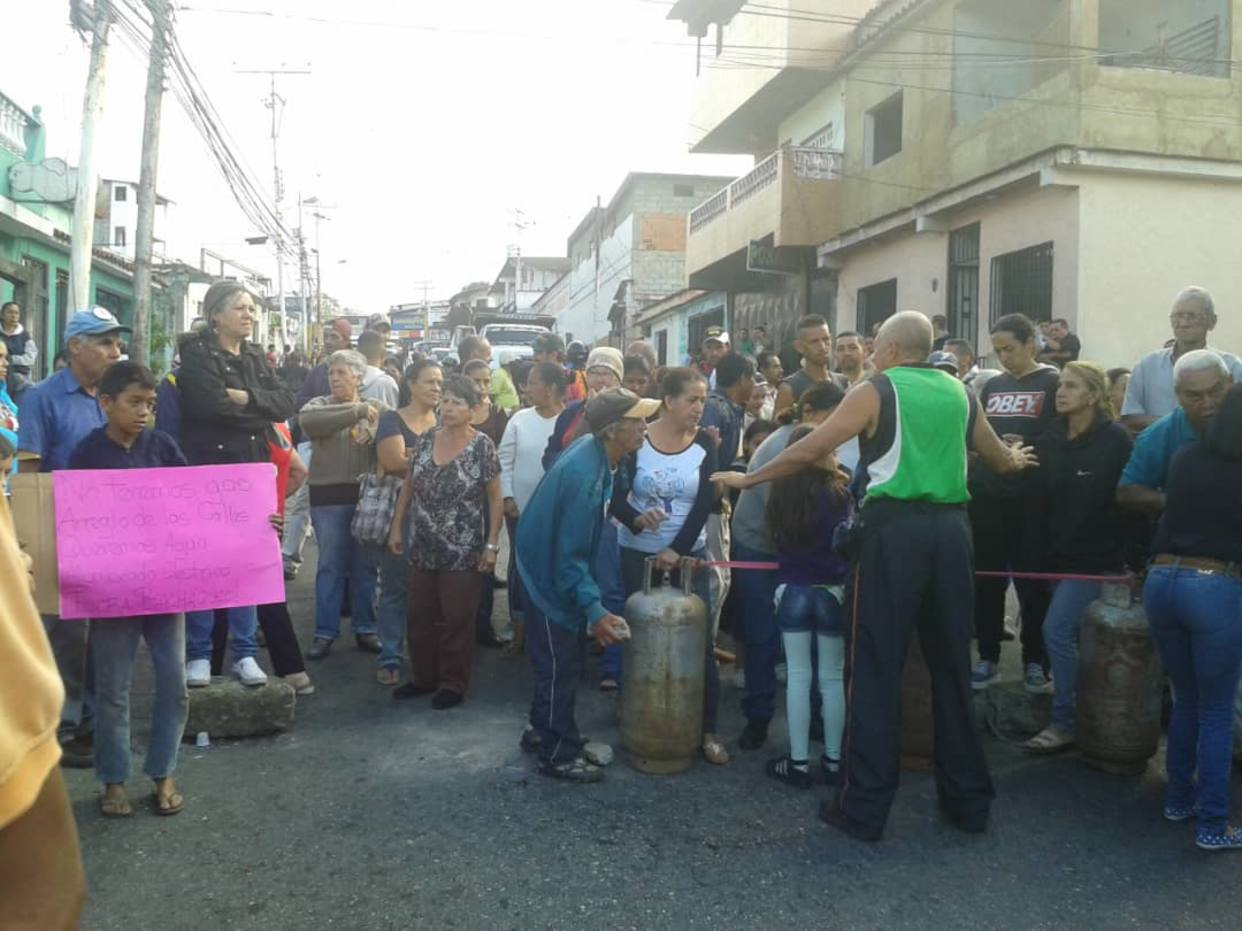
\includegraphics[width=300px]{2.jpg}%
\newline%
%
Las comunidades de Santa Isabel, Los Pantanitos y Primera Sabana de la parroquia El Carmen, estado Trujillo, protestan este jueves por falta de gas desde hace cuatro meses.%
\newline%
%
Reportes de Twitter indican que desde agosto los habitantes~no cuentan con el servicio de distribución.~Imágenes difundidas en la red muestran a los manifestantes en la calle con pancartas.%
\newline%
%
Los afectados también exigen respuesta por el alumbrado, el agua y el estado de las vías.%
\newline%
%
\end{document}